\documentclass{article}%
\usepackage[T1]{fontenc}%
\usepackage[utf8]{inputenc}%
\usepackage{lmodern}%
\usepackage{textcomp}%
\usepackage{lastpage}%
\usepackage[head=40pt,margin=0.5in,bottom=0.6in]{geometry}%
\usepackage{graphicx}%
%
\title{\textbf{Denunciaron torturas al capitán Caguaripano durante su audiencia previa}}%
\author{El Nacional Web}%
\date{16/11/2018}%
%
\begin{document}%
\normalsize%
\maketitle%
\textbf{URL: }%
http://www.el{-}nacional.com/noticias/presos{-}politicos/denunciaron{-}torturas{-}capitan{-}caguaripano{-}durante{-}audiencia{-}previa\_260099\newline%
%
\textbf{Periodico: }%
EN, %
ID: %
260099, %
Seccion: %
Presos políticos\newline%
%
\textbf{Palabras Claves: }%
Política, Presos políticos\newline%
%
\textbf{Derecho: }%
1.2%
, Otros Derechos: %
1.3%
, Sub Derechos: %
1.2.2, 1.3.1%
\newline%
%
\textbf{EP: }%
NO\newline%
\newline%
%
\textbf{\textit{El capitán fue aprehendido el 11 de agosto de 2017 por efectivos policiales en el municipio Sucre de Caracas, y su audiencia había sido diferida hasta este viernes}}%
\newline%
\newline%
%
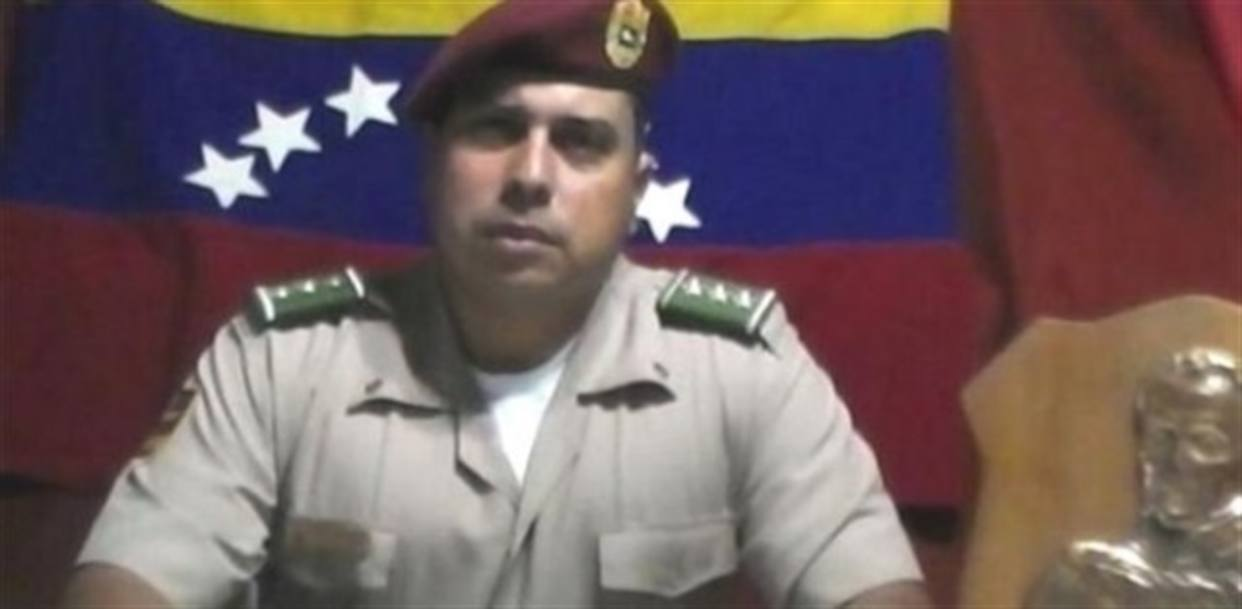
\includegraphics[width=300px]{58.jpg}%
\newline%
%
La Coalición por los Derechos Humanos y la Democracia, organización no gubernamental de abogados defensores de civiles y militares, informó que este jueves que concluyó la audiencia preliminar del capitán Juan Carlos Caguaripano Scott y de otros miembros del cuerpo castrense del caso Paramacay.%
\newline%
%
Susana Rojas, miembro de la coalición, reiteró que el debido proceso del militar detenido fue violentado desde su detención.%
\newline%
%
"Ahora el pasa a juicio. Indudablemente que el debido proceso fue completamente violentado. Ha pasado demasiado tiempo~desde la fecha en que fue detenido, y es ahora que les hace la audiencia preliminar", explicó Rojas a~El Nacional Web.%
\newline%
%
La defensora de los derechos humanos aseguró que el abogado de Caguaripano está "muy impactado" por las torturas físicas y psicológicas que le han infligido a Caguaripano.%
\newline%
%
"Debemos recordar que él era uno de los que estaba detenido en La Tumba, un calabozo en la sede del Servicio Bolivariano de Inteligencia Nacional (Sebin) en Plaza Venezuela", indicó.%
\newline%
%
El capitán fue aprehendido el 11 de agosto de 2017 por efectivos policiales en el municipio Sucre de Caracas, y su audiencia había sido diferida hasta este viernes.%
\newline%
%
La organización no gubernamental indicó, en Twitter, que~de 402 presos políticos registrados en Venezuela, 163 son militares.%
\newline%
%
\end{document}